\section{ACS, 1394-fin, and Wafer Stepper}
The ACS Manager along with Containers and Components is a part of the software of the ALMA project, carried out by the European Southern Observatory~\cite{ploeger.alma}.
The intention of this project is to put more than 60 radio telescopes on a plane high up in the mountains of Chili for radio astronomy.
A specification of this system is part of the official distribution of the \mCRLTwo toolset~\cite{mcrl2}.
Figure~\ref{fig:prop-pres-case-studies:acs-rules} describes a transformation of the receive action (\action{rcv}) into a more detailed procedure involving decompression of the received message.
This rule was applied on the two components and one container present in the specification.
The other parties in the two-way synchronizations were essentially left unchanged.
However, by rewriting the action~\action{send} to $\action{send}'$, we ensure that the rule system is terminating, confluent, and synchronization uniform.
Furthermore, the rule system adds a synchronization rule stating that \action{decompress} can be fired by itself.

\begin{figure}[hbt]
\centering
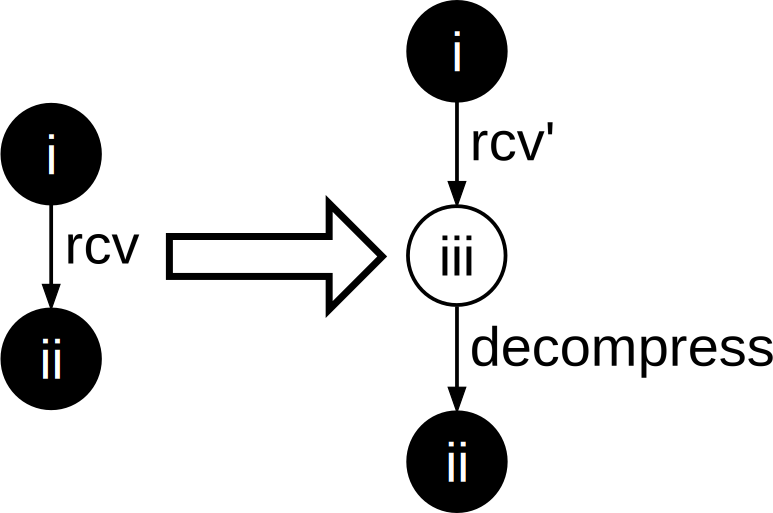
\includegraphics[scale=0.2]{prop-pres-case-studies/figs/acs-rules}
\caption{A transformation rule refining the processing of received messages}
\label{fig:prop-pres-case-studies:acs-rules}
\end{figure}

The 1394-fin (Firewire) case and the Wafer Stepper case are two other \mCRLTwo specifications that have been transformed using rules very similar to this rule, but which involve different numbers of transitions.